\subsection{Experimental setup}

\frame{\frametitle{Experimental setup}
	\centering
	Validation on a \textit{leave-species-out} scheme \\ \vspace{8pt}
	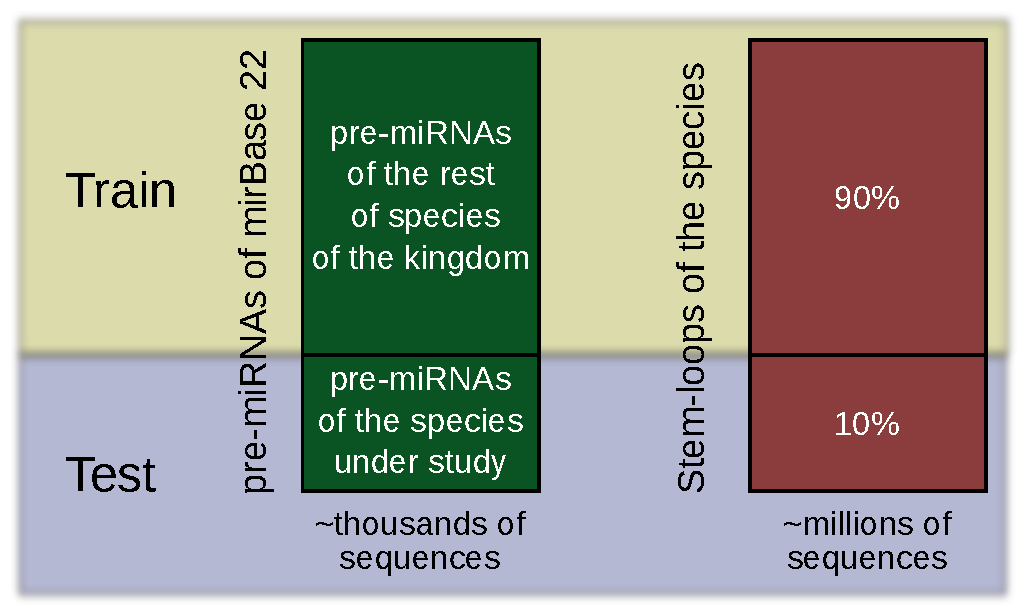
\includegraphics[width=\textwidth]{res/partitions.pdf}
}


\frame{\frametitle{Experimental setup}
\begin{itemize}
	\item Test on three well-known species: \textit{Arabidopsis thaliana}, \textit{Caenorhabditis elegans} and \textit{Anopheles gambiae}. \vspace{8pt} \pause
	\item Two machine learning methods and one sequence alignment method were used for comparison. \vspace{8pt} \pause
	\item The precision and recall were used as performance measures: \vspace{8pt} \\
		\begin{center}
			$Pr = \frac{TP}{TP+FP}$ \hspace{8pt} $Rc = \frac{TP}{TP+FN}$ \vspace{8pt}
		\end{center} \pause
	\item Varying the threshold that defines what is classified as positive or negative, precision-recall curves were generated.
\end{itemize}
}

\subsection{Precision-recall curves}

\frame{\frametitle{Precision-recall curves}
\includegraphics<1>[width=\textwidth]{res/PRROC-ath1.pdf}%
\includegraphics<2>[width=\textwidth]{res/PRROC-ath2.pdf}%
\includegraphics<3>[width=\textwidth]{res/PRROC-cel.pdf}%
\includegraphics<4>[width=\textwidth]{res/PRROC-aga.pdf}
}

\frame{\frametitle{Area under the curves}
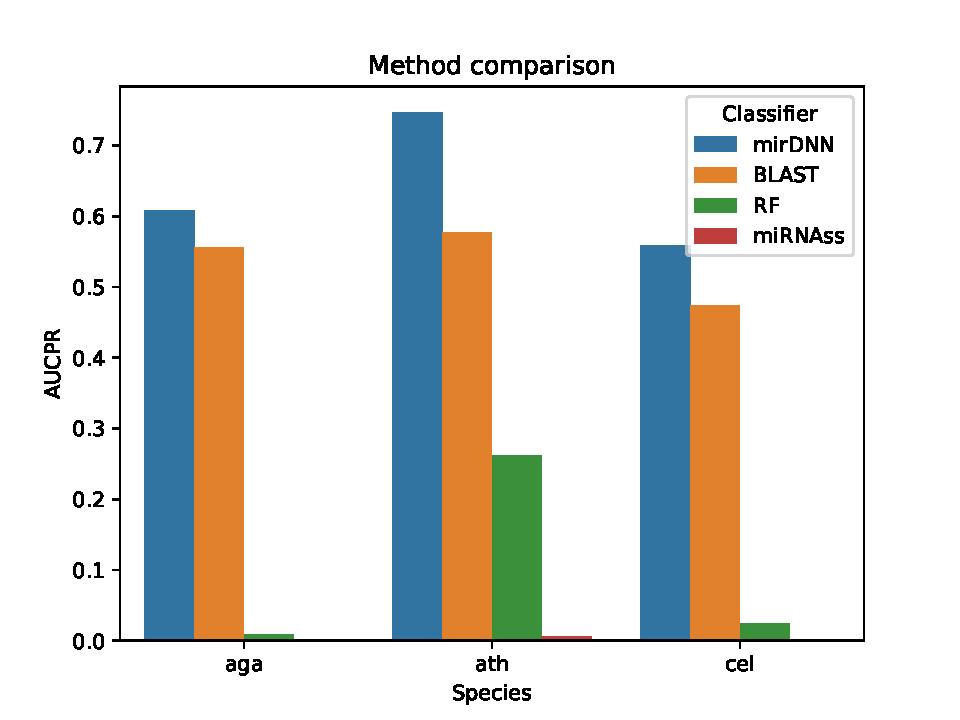
\includegraphics[width=\textwidth]{res/barplot.pdf}
}

